\chapter{Literature Review}\label{ch:Background}

This chapter provides some background research on the project and examines some work carried out in the area of research. Firstly, the chapter will give an overview of Machine Learning in general, then supervised machine learning will be discussed in greater detail. The chapter will then focus on the use of Machine Learning in the Healthcare sector and the work currently being done in this area. Finally the challenges that arise with the use of machine learning with healthcare related datasets will then be explored. This review does not claim to be exhaustive or systematic and instead focuses on work achieved in recent years, while trying to compare several examples of work that has been done in the field and discuss their reach and limitations.

\section{Machine Learning}
Machine learning is considered to be a branch of artificial intelligence and has been around for decades. It has been defined by Arthur Samuel as ''the programming of a digital computer to behave in a way which, if done by human being or animals would be described as involving the process of learning'' \citep{Samuel:1959vp}.\newline 
Technological advances since then have meant that considerable amount of data have been produced and will need to be analyzed. A report by the EMC corporation estimates that newly generated data will grow 40\% a year and that by 2020, the size of the ''digital universe'' will reach 44 zettabytes \citep{EMC:ylTs53OV}. Despite the larger quantity of data being produced daily, as of 2013, only 22\% of the data generated worldwide was considered useful if it were tagged, and less than 5\% was actually analyzed. It is estimated, however that proportion of the data considered useful is likely to reach 35\% by 2020, mostly due to the growth of data from embedded systems \citep{EMC:ylTs53OV}.\newline
This growth in data production and the advances in computing generally means that the field of machine learning and artificial intelligence have also seen growth and are expected to continue growing \citep{Colombus:wm}. Recent decades have seen sharp increases in computing speed, in turn allowing systems to collect and process large quantities of data very rapidly \citep{Denning:2016fz}.\newline
At the same time as computing power increased, the cost of both transistors and storage have decreased markedly: from \$222 per million transistors in 1992 to \$0.06 per million transistors in 2012 and from \$569 per gigabyte of storage in 1992 to \$0.03 per gigabyte in 2012 \citep{Hagel:2013ur}. These two factors combined with increased availability of competent graduates in the field of AI as well as cultural acceptance from the public have allowed the field of machine learning to expand \citep{Evans:sHGdqFvY}. Indeed in 2017, Deloitte predicted that 300 millions smart phones would have on-board neural network machine learning capabilities, meaning that pattern recognition could happen in some instances (e.g. language translation, navigation) without network connectivity \citep{Deloitte:2017wo}.\newline

Although machine learning represents a number of algorithms, it can be broadly categorized in two types: supervised and unsupervised learning (see figure 2.1). In supervised learning, the learning agent will observe some example input-output pairs and learns a function that maps from input to output \citep{Russell:2016tz}. In other words, the goal of supervised learning is to learn a function that can best approximate the relationship between input and output observable in the data \citep{Mullainathan:uy}.\newline 
In contrast, in unsupervised learning, the tasks are generally clustering, representation learning or density estimation(see figure 2.1), i.e. learning the inherent structure of the data without explicitly-provided labels. The lack of labels means that there is no specific way to measure model performance in unsupervised learning \citep{Soni:tr}.

\begin{figure}[H]
\centering
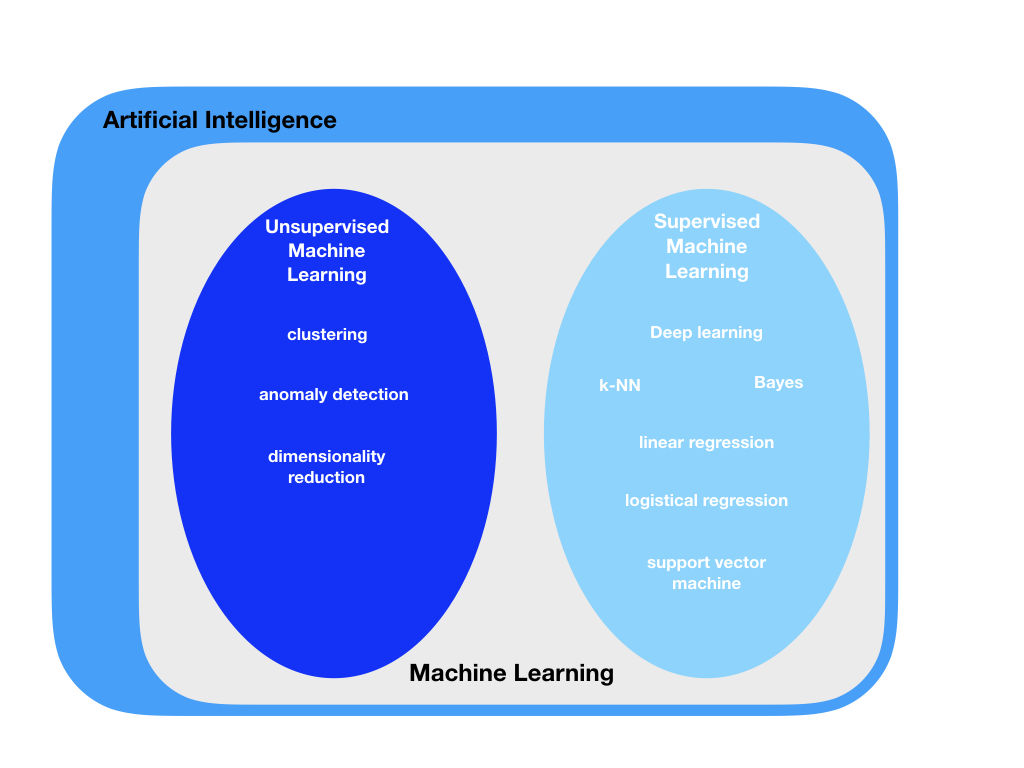
\includegraphics[width=0.8\textwidth]{ThesisTemplate/usingLatex/images/Figure1.png}
\caption{Types of machine learning: this diagram shows examples of algorithms for machine learning and which category they belong to.}
 \label{fig:machineLearning}
\end{figure}


Machine learning is used in many different sectors from finance to healthcare, through to education and customer relations. Many machine learning algorithms are now used to assist decision making in many fields (e.g. credit scoring \citep{Guegan:2018ey}, medical diagnosis) with many having shown very high performance (Figure 2.2. shows investment in AI (which comprises machine learning) generally by sector).

\begin{figure}[H]
\centering
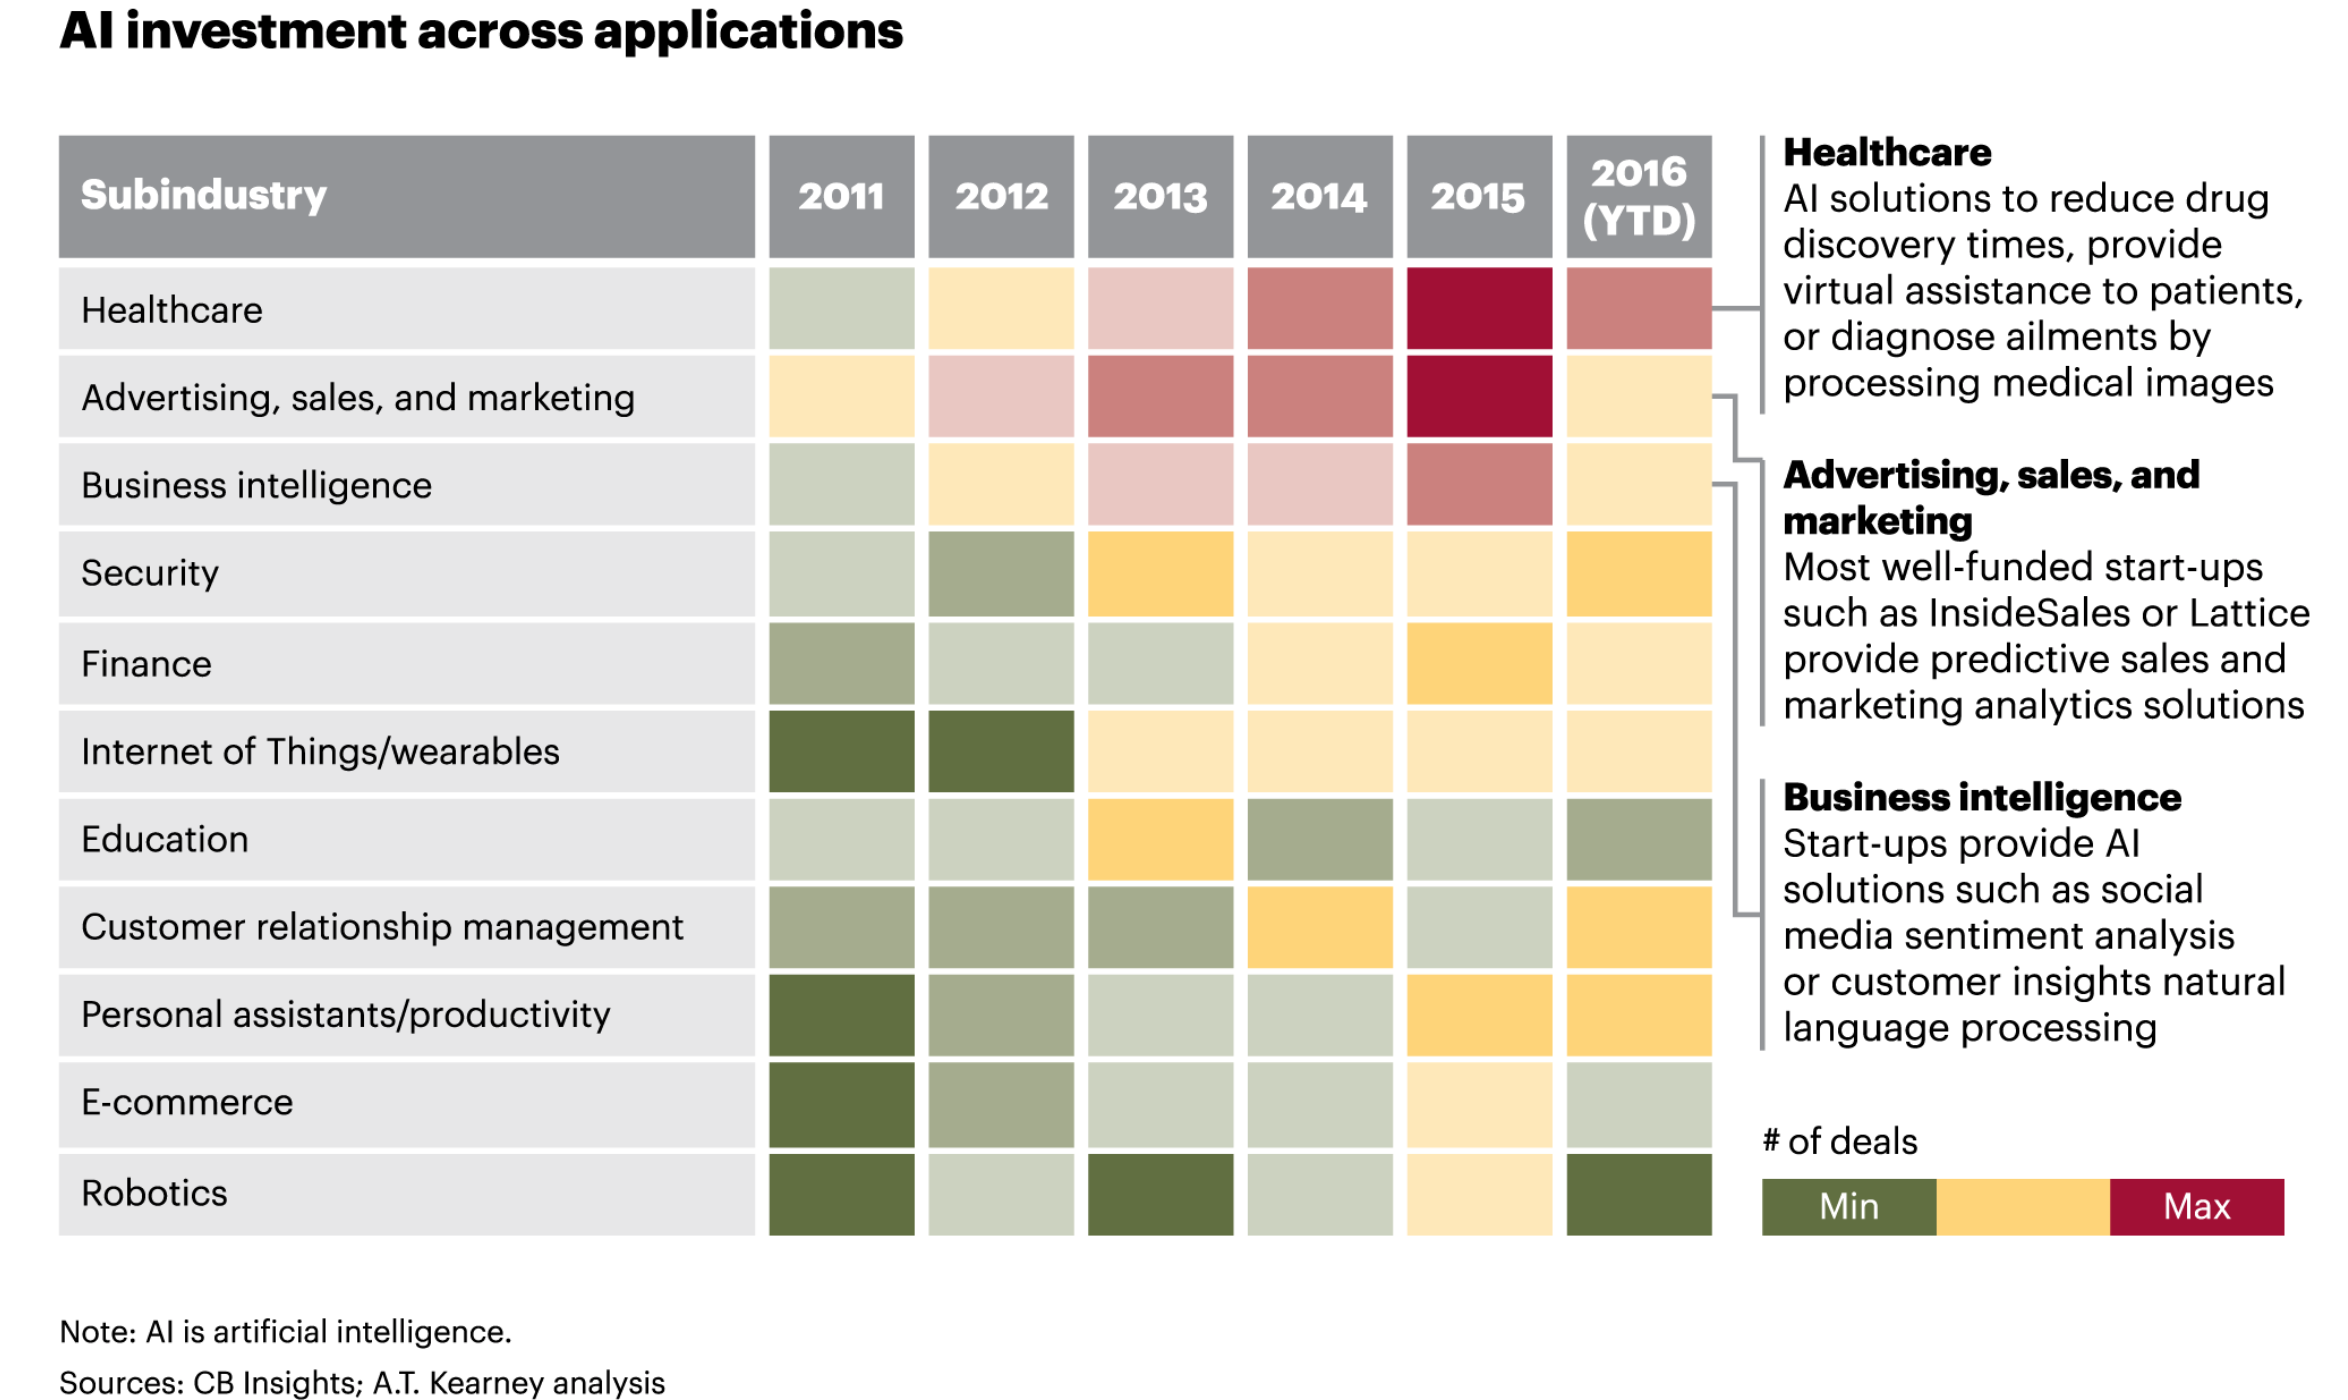
\includegraphics[width=0.8\textwidth]{ThesisTemplate/usingLatex/images/fig2_2.png}
\caption{Investment in AI by sector (source: Will you embrace AI fast enough? \citep{Evans:sHGdqFvY}}
\label{fig:investement}
\end{figure}

It is important however to point out that each algorithm will have a True Positive (TP) rate, a False Positive (FP) rate, a True Negative (TN) rate and a False Negative (FN) rate \citep{Ting:2016ue}:
\begin{itemize}
    \item The TP rate is the proportion of correctly identified instances for positive condition of the target label. For example in the case of a given medical diagnosis, TP would be the number of correctly identified sick patients for a given condition.
    \item  FP is the proportion of incorrectly labelled instances for the positive condition of the target label, i.e the number of actually negative instances that have been labelled as positive by the algorithms. 
    \item TN is the proportion of correctly labelled instances for the negative condition of the target label, i.e. how many healthy patients have been appropriately labelled as healthy.
    \item FN is the proportion of incorrectly labelled instances for the negative condition of the target label, i.e. how many sick patients were labelled as healthy by the algorithm.
\end{itemize}

These figures are used to estimate the performance of a given algorithm (more in section 2.2.2) and these parameters must be known when real life decisions are being made. \newline For very high performing algorithms, there is an increased chance of false positives, which could have unintended real-life consequences (for example in the field of medicine, if a diagnosis of serious illness is made by the algorithm but the patient is healthy, they may have to undergo unnecessary tests to confirm the diagnosis). \newline 
Equally, an algorithm with lower performance will have a higher rate of false negatives which could also have dire consequences (e.g. mislabelling sick individuals as healthy). Thus there are ethical and moral considerations to be taken into account when machine learning algorithms are developed for decision making with real life implications.\newline 

\section{Supervised Machine Learning}
\subsection{Definition}
Supervised learning is typically carried out in the context of classification (mapping input to output labels) or regression problems (mapping input to continuous output). In both cases, the aim is to establish a specific relationship in the input data that will allow the output data to be correctly labelled \citep{Soni:tr}. 

\begin{figure}[H]
    \centering
    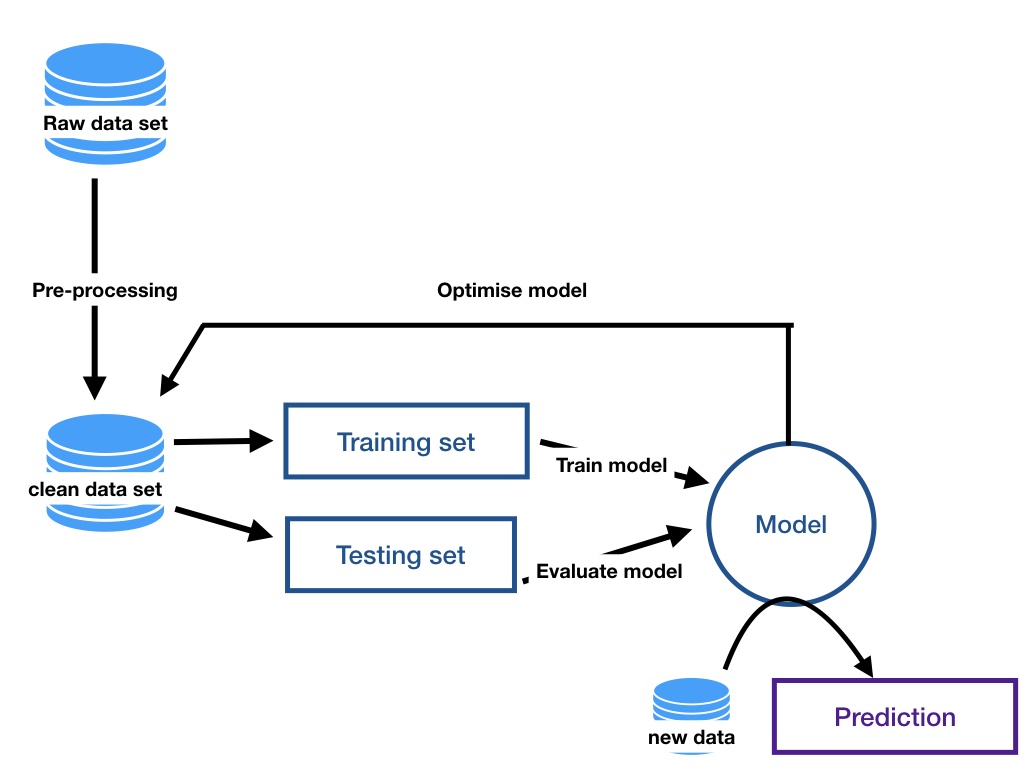
\includegraphics[width=0.8\textwidth]{ThesisTemplate/usingLatex/images/supervisedLearning.png}
    \caption{An example workflow of the supervised learning process. Pre-processing refers to any treatment of the data before it is used to train the algorithm and can include normalising, imputing or scaling.}
    \label{fig:supervisedLearning}
\end{figure}


\subsection{Evaluating Performance and challenges}

\subsubsection{Performance evaluation}
There are many ways to evaluate the performance of a supervised learning algorithm. In section 2.2.1, the TP, FP, TN and FN numbers were explained and these are used in a number of the metrics that have been developed to assess the performance of a given algorithm.

Although there are additional ways to assess the performance of an algorithm, this section will discuss the following: accuracy, calibration, discrimination, negative predictive value, precision, recall and specificity \citep{Callahan:2017bz}.

\begin{enumerate}
    \item Accuracy \newline
    The accuracy of a model is defined as the number of correct predictions made by the model (i.e. TP and TN) divided by the total number of predictions made.
    
    \begin{equation}
        A = \frac{TP + TN}{TP + FP + TN + FN}
    \end{equation}
    
    \item Calibration\newline
    This is a measure of how closely predicted probabilities for an outcome match the observed outcome in test data, also known as the Brier score
    
    \begin{equation}
        Brier score = \frac{1}{N} \sum_{i=1}^{N} (p_{i} - o_{i})
    \end{equation}
    
    \item{Discrimination}\newline
    Discrimination is a measure of how well a model discriminates between randomly selected true positive cases and true negative cases, usually measured as the area under the receiver operator curve (AUC).
    
    \begin{figure}[H]
    \centering
    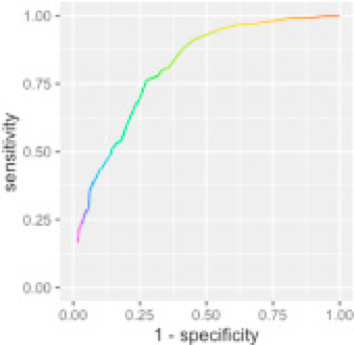
\includegraphics[width=0.5\textwidth]{ThesisTemplate/usingLatex/images/AUC.png}
    \label{fig:aucLearning}
    \end{figure}
    
    \item{Negative Predictive Value}\newline
    This is obtained by dividing the total number of correct negative classifications made (TN) by the total number of negative classifications (TN + FN).
    
    \begin{equation}
        NPV = \frac{TN}{TN+FN}
    \end{equation}
    
    \item{Precision or Positive Predictive Value}\newline
    Precision is the total number of correct positive classifications made (TP) dividided by the the total number of positive classifications made (TP + FP).
    
    \begin{equation}
        P (or PPV) = \frac{TP}{TP + FP}
    \end{equation}
    
    \item{Recall or Sensitivity}\newline
    This metric is also known as the true positive rate and is calculated by dividing the total number of correct positive classifications made (TP) by the number of positive class members in the data (TP + FN).
    
    \begin{equation}
        R = \frac{TP}{TP+FN}
    \end{equation}
    
    \item{Specificity}\newline
    This metric is also known as the true negative rate and is obtained by dividing the total number of correct negative classifications made (TN) by the number of negative class members in the data (TN + FP).
    
    \begin{equation}
        S = \frac{TN}{TN+FP}
    \end{equation}
    
\end{enumerate}

\subsubsection{Challenges in supervised machine learning}
\begin{enumerate}
\item{The bias-variance tradeoff:}\newline
An important concept in supervised learning is that of bias-variance trade-off. The bias variance decomposition is a useful tool to understand the performance characteristics of a learning algorithm. The  mean squared error of a model is made up of the bias and the variance. Bias indicates how accurate the model is on average across different training sets. The variance indicates how sensitive to small changes in the training data the learning algorithm is \citep{Sammut:2016gd}.

\begin{equation}
        MSE = bias^2 + variance
\end{equation}

Thus, any effort to reduce the variance will increase the bias and vice versa. Typically, a model with large bias and low variance will have a tendency to overfit as shown in figure . Linear Regression, Linear Discriminant Analysis and Logistic Regression are all example of algorithms which exhibit high bias and low variance \citep{Anonymous:2016um} whereas Decision Trees, k-Nearest Neighbors and Support Vector Machines exhibit low bias and high variance \citep{Anonymous:2016um}.

\begin{figure}[H]
    \centering
    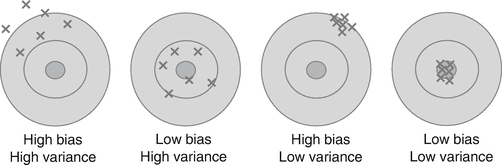
\includegraphics[width=0.8\textwidth]{ThesisTemplate/usingLatex/images/biasvariance.png}
    \caption{Bias-Variance trade-off (Adapted from \citep{Sammut:2017vv}): the optimal scenario is that of the furthest right target, although in practice this is difficult to obtain; Models displaying high bias and low variance will be more uniform but less accurate(third target) whereas models with low bias and high variance will be more accurate but less uniform. The least optimal scenario is that of a high bias and high variance.}
    \label{fig:biasVariance}
\end{figure}

In supervised learning, model complexity and bias-variance trade-off have to be considered and they are in fact interrelated. Typically an overly simple model with few parameters will display high bias and low variance \citep{Anonymous:vm} but a complex models with many parameters will show low bias and high variance, thus it is important to find the right balance of complexity as determined by the bias-variance tradeoff.

\item{The class imbalance problem:}\newline
A dataset is said to suffer from a class imbalance problem when the class distributions are highly imbalanced i.e. one class is greatly underrepresented \citep{Ling:2017jm}. This can lead many classifiers to have low predictive accuracy for the infrequent class. It is assumed that in a two-class case, the minority class is the positive class and the majority class is the negative class. In many real life cases (e.g. medical applications), the minority class could be as infrequent as 1\% of the dataset, thus if a cost-insensitive classifier were applied to the data, it is highly likely that the classifier would predict everything as negative. This is of particular interest in real-life applications where either the goal of the classifier is not to maximise accuracy or the class distribution of the training and test sets are very different \citep{Ling:2017jm}.\newline
If the cost of different types of error (i.e. that of False Positive versus that of False Negative) for a classifier is not the same a cost-sensitive learning algorithm can be used instead \citep{Ling:2017jm}.\newline
In the case of different class distribution between the training and testing data, one approach can be to sample the training data in such a way that its class distribution matches that of the test data; this can be achieved by over-sampling of the minority class and under-sampling of the majority class. \newline
Another approach is to split the minority and majority class into sub classes that relate to the original classes. For instance if the majority class was Healthy (H) and the minority class Sick (S), they could be further divided as VH (very healthy), H and BH (borderline healthy) and BS (Borderline sick), S and VS (very sick). This implies a good knowledge of the domain but has the advantage that LS, S and VS are all scored as positive and VH, H and BH are all scored as Healthy, which may improve the accuracy of the algorithm by reducing the class imbalance (Eyad Elyan, personal communication).\newline
\end{enumerate}

\section{Machine Learning in Healthcare}
\subsection{Motivation: data in healthcare}
One key area where machine learning is being invested in is the healthcare sector \citep{Obermeyer:2016ju,EMC:2014ve, Evans:sHGdqFvY}, see figure 2.2. Indeed data growth in this sector has been growing at a faster rate than other sectors (48\% annual growth versus 40\% growth on average for other sectors) according to a report from EMC \citep{EMC:2014ve}. And it is thought that new healthcare applications will drive data growth. For example, the adoption of Electronic Health Record (EHR) in the United States by healthcare providers (hospitals, GP) is growing so fast that it is estimated that by 2020, penetration of EHR in the US market will reach 95\%. Further, increasingly stringent regulations of data protection and maintenance, especially in the healthcare sector means that many providers choose to keep data indefinitely \citep{EMC:2014ve}. However large amounts of this data is still largely unused and according to the EMC corporation, better data analytics will help identify the most useful data, which will in turn enable information-driven decision.\newline
The healthcare sector also faces challenges in most parts of the world. Firstly, the global population is ageing. According to data collected by the United Nation Department of Economic and Social Affairs (Population Division), the number of older persons (60 years or over) is estimated to more than double by 2050, rising from 962 million globally in 2017 to 2.1 billion in 2050, meaning that population aged 60 or over is growing faster than all younger age groups \citep{UnitedNations:2017wd}. An ageing population with longer life expectancy will make more demands on the health services everywhere. A second challenge of the sector is the shortage of physicians and other care providers. For example in the United States, the number of primary care physicians is expected to increase by only 8\% whereas the demand for primary care physicians will rise by 14\% resulting in a shortfall of around 20, 400 physicians \citep{EMC:2014ve}. The trend is similar in the UK and other European countries \citep{Campbell:ti}. At the same time, patient expectations will increase as people will expect treatments and care in line with technological developments.\newline
Together these factors  mean that the healthcare sector needs to adapt and to be able to deliver care in the most efficient way and will need to turn to Information Technologies in general to help scaling the process, and to machine learning in particular in order to facilitate a greater output of robust diagnosis, uncover novel drug candidates, or detect best possible treatment given a patient's background.\newline

\subsection{Opportunities for the use of machine learning in healthcare: what problems can be solved?}
Although the use of machine learning in healthcare is not new (there are many commonly used teaching healthcare-related datasets from studies done in the 1980s and 1990s; the Breast Cancer Dataset for example was first used in a study published in 1994 \citep{OLMangasarian:1994ue} and the Pima Indian Diabetes dataset was used in a study from 1988 \citep{Smith:1988wy}), recent years have seen an increase in publications relating to machine learning and healthcare, most likely driven by the general growth in machine learning centred research as discussed in the previous section but also by the increasing volume of data being produced \citep{Pesapane:2018kv}. Figure 2.5 shows the increase in publications which were found in EMBASE by using terms such as machine learning or deep learning and radiology, showing an 8-fold increase since 2006. A search in Google Scholar with the terms "Machine Learning" and "Healthcare" for articles published between 2016 and 2018 returned 978 results.\newline

\begin{figure}[H]
\centering
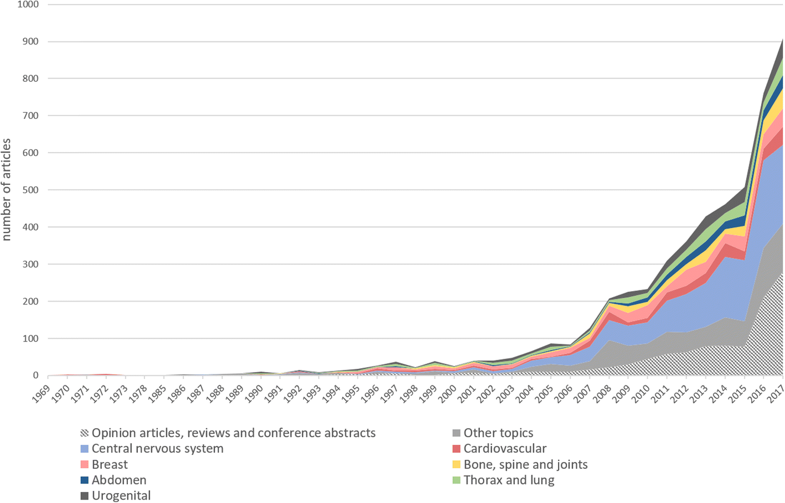
\includegraphics[width=0.7\textwidth]{ThesisTemplate/usingLatex/images/PesapaneFig.png}
\caption{Figure from \citep{Pesapane:2018kv}: Number of publications indexed on EMBASE obtained using the search query ('artificial intelligence' OR 'artificial intelligence' OR 'machine learning' OR 'machine learning' OR 'deep learning' OR 'deep learning') AND ('radiology' OR 'diagnostic imaging'). EMBASE was accessed on April 24, 2018. For each year, the number of publications was subdivided separating opinion articles, reviews and conference abstracts from original articles in seven main subgroups considering subspecialty or body part. Other fields of medical imaging different from those listed above are grouped under the 'other topics' label (e.g. dermatology, ophthalmology, head and neck, etc.)}
\label{fig:publications}
\end{figure}

The previous chapter discussed briefly the potential of machine learning to greatly help in the field of epidemiology by providing an alternative to randomised control trials (RTC) or case-control studies by exploiting large patient datasets which are now available in electronic format across large geographical areas \citep{Callahan:2017bz}, through the adoption of EHR. Studies where machine learning has been applied to EHR are increasingly popular \citep{Goldstein:2017bk}.\newline 
EHR data differ from the traditional cohort based risk-studies since the data may not be standardised, is generally collected more frequently and is collected without the use strict inclusion requirements.\newline
There are advantages to the use of EHR data as they are typically collected more often than those from cohort studies and will more often reflect real-world situations than the data obtained from restrictive cohort studies. In one such case, a model to predict heart failure survival was built using EHR data from the Mayo Clinic \citep{Panahiazar:2015gp}. The authors compared their model to the existing Seattle model and found that the use of EHR data provided a model that was more accurate (11\% AUC improvement) and more convenient to use in a clinical setting. Panahiazar and colleagues suggested that one of the reasons their model showed better predictions than the existing one is that the Seattle Heart Failure Model (SHFM) is extrapolated from clinical trial databases and therefore does not always reflect real-life situations.\newline
There are many more areas where machine learning could improve healthcare delivery such as the stratification of patients into risk category or to characterise and predict a variety of health risk, as well as early diagnosis of certain conditions. The literature abounds with examples of successful machine learning algorithms which have been developed with these goals in mind.\newline 
Traditional risk scoring systems can be flawed as some of the features used to compute the score may not reflect a wide enough variety of the population \citep{Besseling:2017bs}. Those limitations have led several groups to turn to machine learning to build robust statistical models that will classify individuals appropriately and provide accurate level of risks \citep{Callahan:2017bz, Besseling:2017bs}.\newline
Several research groups have successfully developed algorithms that outperformed existing stepwise logistic regression models to predict the risk of mortality of an individual or to diagnose a condition in a patient. For instance  Ross and colleagues developed a machine learning algorithm to identify the presence of peripheral artery disease (PAD) and predict future mortality risk \citep{Ross:2016kh}.The data used in this study was derived from a prospective observational study with a view to identify key demographic, clinical and genomic factors that differs between those presenting with PAD and those that do not. The disease was not used as a factor for enrolling patients in the study, however patients enrolled included those referred for complaints of angina, dyspnea or had abnormal stress results. Clinical data were obtained at enrolment and patients were followed for observation of any adverse event. Therefore there is a small element of bias in the sample used to build the algorithm, although the presence of PAD was not known at enrolment, the patients were already being enrolled in a study because of a number of complaints.\newline
 To build the model, the researchers included any variable for which a majority of patient had a data value. In other words, no variable was included based on \textit{a priori} hypotheses and patients were included if they had complete data. The researchers were able to build a Random Forest-based algorithm that successfully identified undiagnosed PAD (AUC:0.84). The model was also used to predict mortality (AUC:0.76). PAD is highly prevalent as well as difficult to diagnose, so this algorithm could prove very useful in a clinical setting.\newline
 Despite the algorithm performance, there are several limitations to this study. Firstly the algorithm was constructed using only those patients with complete data. This is problematic for clinical application, as patient records are often incomplete (as discussed previously) for a variety of reasons. The authors suggest the possible imputation of data in cases of missing values \citep{Ross:2016kh}. As previously mentioned, the population used to train the algorithm is already considered  to be high-risk, thus the algorithm may not generalise well to other populations.\newline
 Other efforts at patient risk classification have been made  and by other groups have included the application of machine learning to the selection of individuals for genetic testing for familial hypercholesterolemia (FH) \citep{Besseling:2017bs} in an attempt to improve current selection criteria which tend to misclassify certain population, especially young individuals.\newline
 The work carried out by Besseling and colleagues provided a useful model which showed good discrimination and calibration, which compared to existing models allowed for better inclusion of young persons (which the previous models tended to exclude) and this new model is being considered for use in clinical setting. This work allows for the selection of individual for genetic testing which is often expensive and therefore needs to be targeted. The model is to be used on patients with suspicion of FH rather than the population at large.\newline
 Other areas of healthcare where machine learning has been successfully applied include imaging diagnostic, as early as 1994 \citep{OLMangasarian:1994ue} and more recently Aissa and colleagues investigated the impact and clinical performance of a machine learning based tool for the detection of lung nodule in melanoma patients \citep{Aissa:2018jm}.\newline
 The diagnosis of lung nodules is one of the criteria to identify metastases in cancer patients as well as being used for screening of primary malignancies of the lung. The presence of lung nodules in melanoma patients is an indicator of worsen prognosis so its accurate identification is important. In this study the authors compared the reading of CT scans by three radiologists to that of a computer aided detection system (CAD). This novel CAD system is machine learning based and the additional vessel-suppressed reconstruction can be viewed by the radiologist.\newline
 The CAD system did not miss any of the nodules identified by the radiologists also reviewing the images, however the system found additional nodules, which were missed by the radiologists. These turned out to be very small and did not affect therapy. In 9\% of these cases, theses nodules turned out to be false positives and follow up analyses revealed that none of the nodules detected by CAD but missed by radiologist were metastases or would have led to changes of therapy. In 30\% of the cases where the nodules where missed by the radiologist, they were so small that they could not be definitely labelled as benign or not, which means patients needed to be further referred for follow-up. This could lead to further follow-ups and increased costs as well as patient distress. This study suggests that machine learning-aided diagnosis can be of great help particularly in cases where early detection of disease is crucial to patient survival, but the authors stress that findings need to then be reviewed by the appropriate specialists (in this case radiologist) in order to be appropriately interpreted and the CAD system should be used as either second reader or concurrent reader. It is worth noting that the study concerned only a relatively sample size (46 patients) and larger sample sizes may have shown a different false positive result, or the presence of nodules missed by either the CAD system or the radiologists.\newline
 The studies discussed above all show that machine learning can be a powerful tool for diagnostic medicine although there are limitations inherent to the study design or the choice of dataset and these are discussed in section 2.4.\newline
 As previously shown in figure 2.5, Diagnostic Imaging has been a centre of interest for the application of machine learning tools to assist radiologists in their tasks. William and colleagues conducted a review of image analysis and machine learning techniques used for automated cervical cancer screening \citep{William:2018ia}. In total, they reviewed 30 publications from the last 15 years and found that most of the existing algorithms facilitate an accuracy of nearly 93.78\% on an open pap-smear data set, segmented using CHAMP digital image software. K-nearest-neighbors and support vector machines (SVM) algorithms have been reported to be excellent classifiers for cervical images with accuracies of over 99.27\% and 98.5\% respectively when applied to a 2-class classification problem.\newline 
 This review identified some weaknesses in the techniques used, including low accuracy of classification in some classes of cells. Most algorithms documented either worked on single cervical cell images or multiple cervical smear images, not both. The authors suggested that algorithms that can be used on both single and multiple cell images at the same time should be investigated as cells in pap-smear images usually contain overlapping cells.\newline
 The authors also reported that the majority of the algorithms resulted in an accuracy of nearly 93.78\% (still low for diagnosis purposes) and used an open pre-processed pap-smear data set, suggesting that the accuracy of these algorithms could be even lower in a clinical setting, using images that have not already been processed.\newline 
Other areas of the healthcare industry where machine learning could also be useful are numerous and include hospital and practice management, for example to predict demand for emergency department beds or to inform staffing decision \citep{Callahan:2017bz, Tiwari:2014bq}. These applications have the potential to be useful especially in environment for resources are scarce and they present challenges quite different to those centred around patient diagnosis or disease risk predictions. For the purpose of this review, this aspect of machine learning in a healthcare setting will no be discussed further and is only mentioned here for indicative purposes.\newline


\section{Challenges in healthcare}
\subsection{Challenges inherent to the data}
The use of machine learning as applied to healthcare related data is not without challenges. 
Electronic health record data present some difficulties as EHR data is captured for all patients mostly when they are unwell and collect only those metrics that the clinician will think is appropriate for a particular visit, and this can introduce bias in the data \citep{Hersh:2013gp, Goldstein:2017bk}. \newline 
Goldstein and colleagues looked at a large number of EHR and machine learning based studies and analysed both their methodologies and result to  establish areas of weakness and suggestions for future studies to remedy those problems. They identified four main areas where improvements were necessary in order to get the best possible results for EHR based studies: 
\begin{itemize}
    \item Many studies were not carried across multiple centres or did not cross validate using data from another centre, which does not guarantee the portability of the model 
    \item Predictor variables were not always used to the fullest extent of the EHR data and better leverage from the available information could be gained by using time-varying factors
    \item Bias inherent to the data (EHR data contains sicker people on average) is not always addressed, which could in turn affect the robustness of the model
    \item Evaluation metrics were often not suited to the data or the model (c-statistic) and should instead have used Predictive Positive Value or Net benefit metrics. 
\end{itemize}

Conversely, although EHR data tend to be biased towards a higher rate of sick patients, many health-related dataset can be biased towards healthy patients, especially when using cohort-based data. In this case, there are only a small subset of patients with the disease or marker that is being investigated and this can lead to developing models that will easily fail to identify the targeted outcome because the training sets do not contain enough instances of the "sick" label compare to the "healthy" label. This is known as the class imbalance problem and was discussed in section 2.2.2. 
As discussed earlier, this problem can be resolved through stratification of the data or changing from a binary category to a multiple category.
Another common challenge from working with health-related dataset is the problem of missing data. It is especially common when working with EHR \citep{Goldstein:2017bk} but can also happen when working with cohorts and this problem was discussed in several of the examples discussed previously \citep{Besseling:2017bs, Ross:2016kh}.\newline
Both studies resorted to data imputation \textit{i.e} the process of replacing missing data with substituted values. This is often done by replacing the missing values with the median value for that variable. Ross and colleagues even report, although this is not published that imputation of missing data may improve predictive accuracy \citep{Ross:2016kh}.\newline
In the studies described in section 2.3, there were several methodological considerations and limitations that were taken into account by the authors. The inclusion or not of variables towards the final model is one such consideration. Often a stepwise selection, without considering previously known association between candidate predictors and outcome, is used. However this might exclude variables that appear statistically insignificant in a multivariable model but would be significant when used in another cohort and may therefore impact the portability of the model. In contrast, by using only variables that have been previously shown to contribute to the outcome while ignoring those that show association in the data, the model risks missing important associations that are yet to be identified \citep{Besseling:2017bs}. To avoid either of these pitfalls, Besseling and colleagues chose to use a two-step approach in choosing the candidate predictors: 
 \begin{itemize}
 \item firstly all variables considered important (based on current literature regarding clinical phenotype of FH) were included in a preliminary model;
 \item then the authors added a combination of eight variables to the model, with a maximum of four added at any time.
\end{itemize}
In contrast the model to identify PAD described by Ross and colleagues \citep{Ross:2016kh} was built by using all variables for which data was available so as to limit deliberate bias in choosing which variables to include in the model.\newline
The size of the dataset used for a study is also of notable considerations as smaller datasets can lead to bias and overfitting  of the data \citep{Steyerberg:2003fq}. Though many studies using machine learning use large datasets, many fail to use multiple centres which may reduce the utility of the model when extrapolated to different population and this has been noted by Goldstein and colleagues \citep{Goldstein:2017bk}. The familial hypercholesterolemia model built by Besseling and colleagues successfully avoided this pitfall using a large training dataset and using an external validation set from a different cohort \citep{Besseling:2017bs}. In the case of the PAD model study, the authors acknowledged that their training size was relatively small and from patients that had been chosen because their data were complete and this could limit use of the model in a clinical setting \citep{Ross:2016kh}.\newline
This also raises another challenge that occurs when developing machine learning in healthcare: class distributions are often very different between the training dataset and the testing datasets. In the case of the study on Familial Hypercholesterolaemia, the algorithm was validated using a testing set that was unrelated to the training set, though the class distribution were similar between the two sets and the two classes were fairly evenly distributed in both sets (40\% and 60 \% in the training set and 45\% and 55\% in the testing set) \citep{Besseling:2017bs}. However, this could be very different in a clinical setting or if the algorithm were to be expanded to a different population where it might be expected the gene mutation may be more or less frequent than in the one used to develop the algorithm. William and colleagues also cites this as a potential problem with many of the algorithms they have reviewed \citep{William:2018ia} since they were trained on commercially, pre-processed images rather than ones obtained from hospitals or clinics.


\subsection{Data access}
Patient level data is considered sensitive data and is therefore protected. In the UK it falls under the Data Protection Act \citep{Government:eUQ8WqXT}  and there are similar laws in place across many other countries.\newline
In order to use patient level data for research purposes, consent of each patient has to be obtained, unless the data is processed so as to be anonymised and collated in such a way that no individual patient can be  identified from their data. In the UK, the CPRD (Clinical Practice Research Datalink, https://www.cprd.com) is responsible for collecting de-identified data from a network of GP practices. This data can be accessed by research groups through an application process \citep{CPRD:VYxcqU74}. Other de-identified data are released by NHS digital for NHS England and by Information Data Service for NHS Scotland.
Other collected-for purposes data can be obtained in the same way as they are obtained for clinical trials. A number of datasets that have been used for published research have now been placed in a de-identified format in the public domain through organisations such as Kaggle(https://www.kaggle.com) or UCI(http://archive.ics.uci.edu/ml/index.php). Many datasets relating to healthcare can be found on these websites and used to create new algorithms or compare the performance of different algorithms on specific datasets.\newline
There are a growing numbers of wearables (Apple Watch, Fitbit, etc) that collect health-related individual data, however these tend to be protected by data protection laws and the various private companies in charge of hosting the data may not share them with researchers unless consent has been explicitly seeked from the user \citep{Apple:nN4TDuuN, Fitbit:FvPrmdk3}. Finally, there has been growing enthusiasm from the public in genomic level data and for profit organisation such as 23AndMe or Ancestry have seen a growing number of customers looking to find out more about their disease risk or ancestry through DNA testing \citep{Regalado:vf}. These companies have various consent policies and will either not share the data or will seek consent of the consumer to share data with selected partners only. 


\subsection{Cultural Challenges: response from healthcare staff and patient}
Although the use of machine learning in the healthcare sector appears to be growing at least in a research setting, its full implementation in clinical setting is still facing some opposition from providers \citep{Cabitza:2017hv}. However some view the growing use of AI and machine learning in healthcare as inevitable \citep{Murdoch:2013hm}, and there are advocates for opening data use in healthcare \citep{Kostkova:2016ur}, with many viewing it as tool which can support rather than replace medical providers \citep{Pesapane:2018kv}.
There are some reticences from patient in sharing their health data for research purposes \citep{Goldacre:tf}, though there is evidence that these attitudes may be shifting \citep{Kostkova:2016ur}. 

\section{Conclusions}
This chapter has reviewed the existing literature relevant to the use of machine learning in the field of healthcare, although the review is in no way exhaustive and has concentrated on aspects of medical diagnosis rather than healthcare management or planning.\newline 
The current level of research in the application of machine learning to healthcare has been increasing in the last decade and the work reviewed in this chapter suggests that machine learning could help the healthcare industry solve some of its staff shortage issues through the partial automation of some of its diagnostic procedure (particularly in the field of imaging). Machine learning could also solve problems in providing patient with the necessary care at the earliest possible time for a given condition through the development of more accurate risk scoring systems. Finally, machine learning could assist with leveraging the ever increasing volume of data generated in the healthcare sector.\newline
These objectives are not without challenges however and the use of machine learning in assisting medical diagnosis can only succeed if those challenges are recognised and addressed appropriately.\newline
First, there are some bias inherent to the data used in healthcare-related studies. These bias need to be addressed during data pre-processing if helpful models are to be developed. Investigating possible solutions to the problem of class imbalance and comparing different way to pre-process the data through feature engineering or other methods may be avenues to improve the performance of algorithms on this type of data.\newline
Second, access to data can be difficult. The development of algorithms using open datasets or carefully recruited cohorts may not yield models that can be deployed across larger populations in a clinical setting and it will be necessary to tap into both EHR data and data obtained from wearables and/or privately requested genomic data through initiatives so that algorithms can be trained on large cross-section of the population.
\newline
A third category of problem broached while reviewing the literature and relating to data access is the issue of consent to use of data, data protection and more generally health provider and patient attitude toward the use of machine learning in healthcare, however this falls outwith the scope of this project and will not be discussed further.\newline




